%settings

\setlength{\parindent}{2ex}
\phantomsection
%text
%-Task1----------------------------------
\section{Model of the application using 3 Activity Diagrams}
In figure \thesection.1 is presented the state chart which contains the output form of my application.
\par
\begin{figure}[h!]
	\centering
	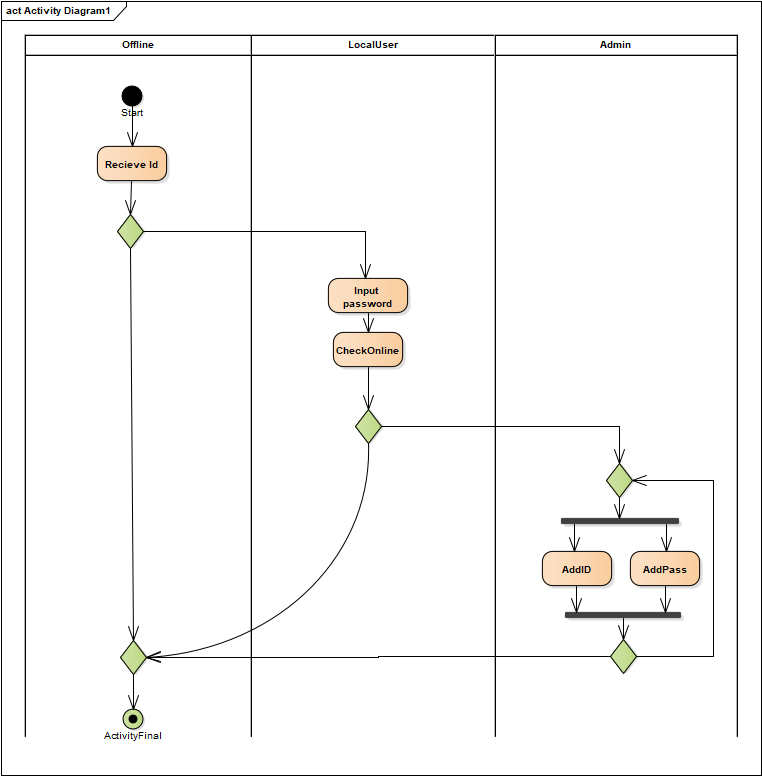
\includegraphics[keepaspectratio=true,scale=0.6]{ActivityDiagram1}
	\caption{Initialization} 
\end{figure}
\par
Here the user chooses if he wants to work online by adding the password and then checking online,after what he can add Id's to track after what he will track these Id's data from selection form.
\newpage
In figure \thesection.2 is presented the state chart which contains the output form of my application.
\begin{figure}[h!]
	\centering
	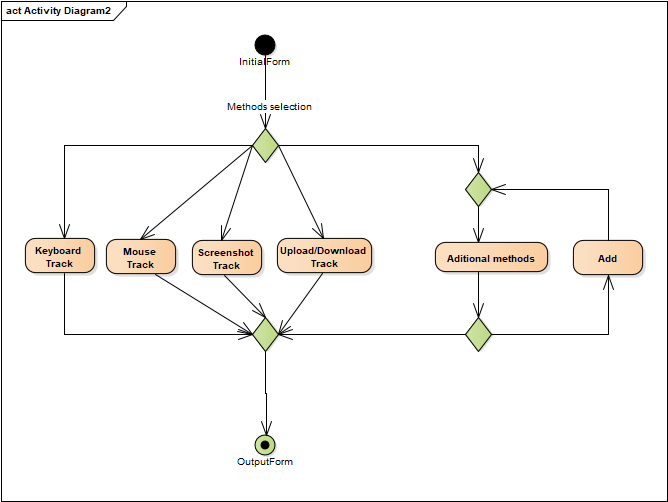
\includegraphics[keepaspectratio=true,scale=0.6]{ActivityDiagram2}
	\caption{Selection} 
\end{figure}
\par
Here user is given methods to select and and continue to work with in the output form.
\newpage
In figure \thesection.3 is presented the state chart which contains the output form of my application.
\begin{figure}[h!]
	\centering
	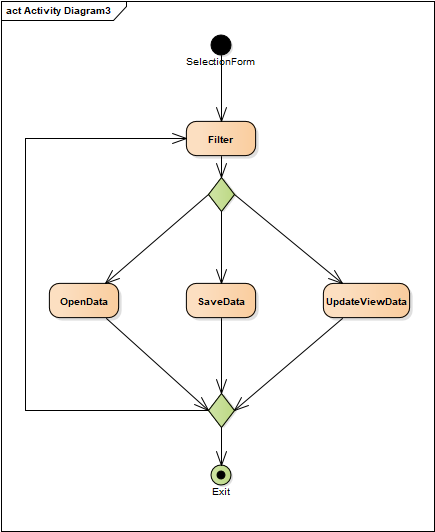
\includegraphics[keepaspectratio=true,scale=0.8]{ActivityDiagram3}
	\caption{Output} 
\end{figure}
\par 
User can choose how to save his data collected from the tacking methods.
%-Task2----------------------------------
\newpage
\section{Activity Map of the application.}
The Activity Map that my application has is based around:
\begin{itemize}
\item[•] Initialization(Where the user selects the mode he wants to operate in)
\item[•] Selection(Where user selects the Tracking methods he wants to use)
\item[•] Output(Where user selects how he wants to output the data that was tracked)
\end{itemize}
\begin{figure}[h!]
	\centering
	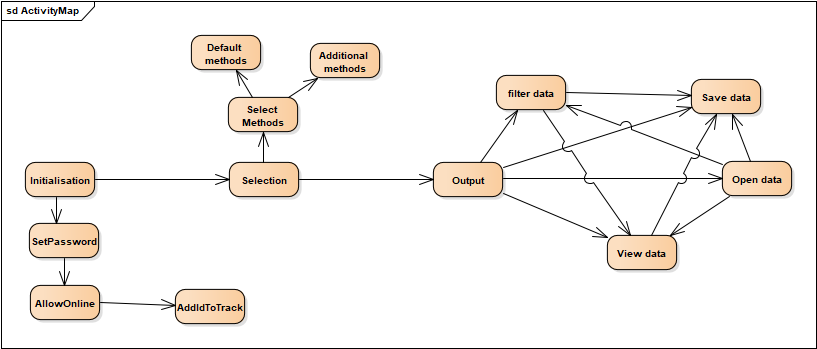
\includegraphics[keepaspectratio=true,scale=0.6]{ActivityMap}
	\caption{Output} 
\end{figure}
\clearpage
